%% Простая презентация с примером включения программного кода и
%% пошаговых спецэффектов
\documentclass[aspectratio=169]{beamer}
\usetheme{SPbAU}
%\useoutertheme{infolines}
\usepackage{fontspec}
\usepackage{xunicode}
\usepackage{xltxtra}
\usepackage{xecyr}
\usepackage{hyperref}
\setmainfont[Mapping=tex-text]{DejaVu Serif}
\setsansfont[Mapping=tex-text]{DejaVu Sans}
\setmonofont[Mapping=tex-text]{DejaVu Sans Mono}
\usepackage{polyglossia}
\setdefaultlanguage{russian}
\usepackage{graphicx}
\usepackage[outputdir=out]{minted}
\usepackage{multicol}
\usepackage{array}

\usepackage{listings}
\setminted[c++]{
  linenos=true,
  fontsize=\footnotesize
}
\lstdefinestyle{mycode}{
  belowcaptionskip=1\baselineskip,
  breaklines=true,
  xleftmargin=\parindent,
  showstringspaces=false,
  basicstyle=\footnotesize\ttfamily,
  keywordstyle=\bfseries,
  commentstyle=\itshape\color{gray!40!black},
  stringstyle=\color{red},
  numbers=left,
  numbersep=5pt,
  numberstyle=\tiny\color{gray},
}
\lstset{escapechar=@,style=mycode}

\begin{document}
\title[Комбинаторы запросов к графам]
{
  Разработка библиотеки комбинаторов запросов к графам
}
\author[Шушаков Д.С.]
{
Шушаков Даниил Сергеевич\\
{\footnotesize\textcolor{gray}{Научный руководитель: Аксенов Виталий Евгеньевич}}\\
{\footnotesize\textcolor{gray}{Научный консультант: Григорьев Семен Вячеславович}}
}
\date{\today}

\frame{\titlepage}

\setlength{\parskip}{0.25cm}

\begin{frame}{Графовое представление данных}
  \begin{itemize}
    \item Данные могут представляться в виде графа и храниться в графовых БД
    \item Вершины и ребра могут иметь свойства
    \item Запрос к графу -- нахождение путей, удовлетворяющих ограничениям
  \end{itemize}
  \center{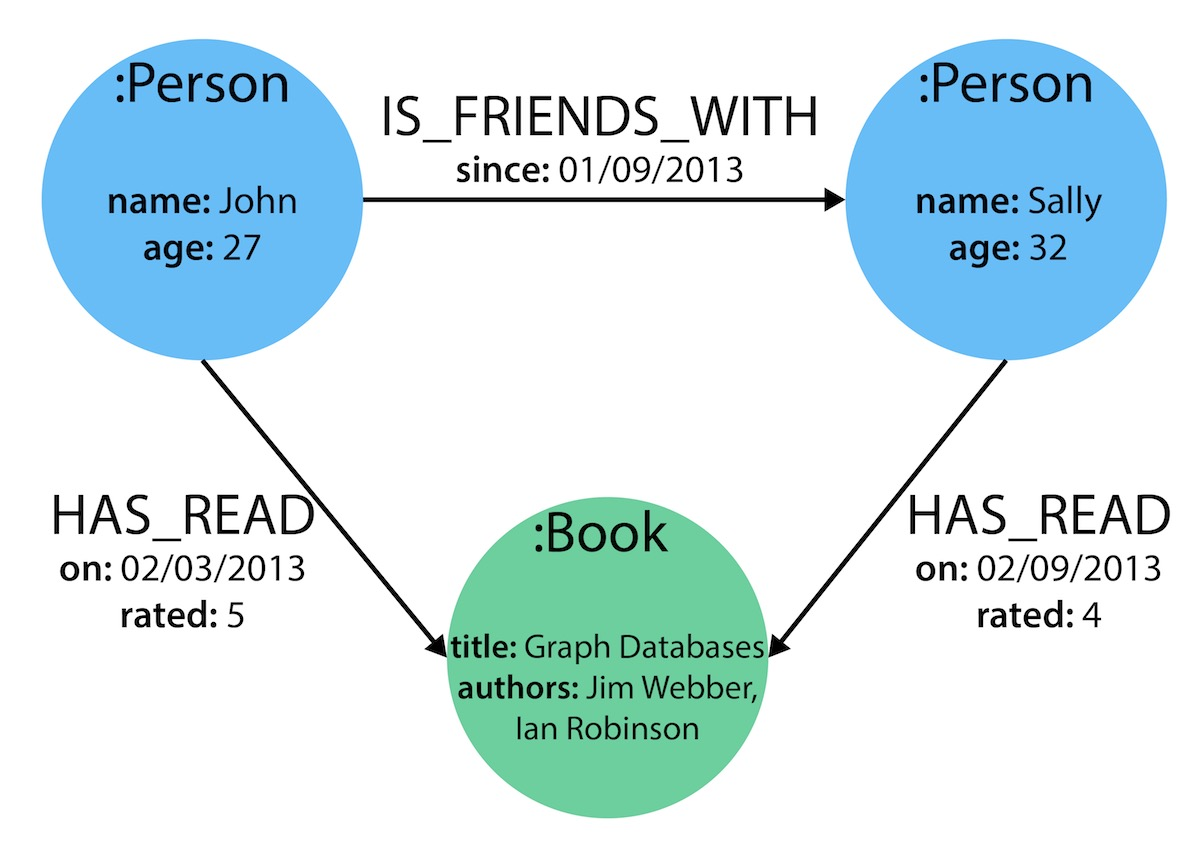
\includegraphics[scale=0.15]{images/gr_example.jpg}}
\end{frame}


\begin{frame}{Строковые языки запросов}
  \begin{itemize}
    \item Для запросов к графам используются строковые языки запросов, например, Cypher для Neo4j
    \item Отсутствие проверки корректности запроса на этапе компиляции
    \item Сложно составлять и переиспользовать подзапросы
    \item Невозможность задать контекстно-свободные ограничения
  \end{itemize}
\end{frame}


\begin{frame}[fragile]{Парсер-комбинаторы}
  \begin{itemize}
    \item Парсер-комбинаторы - функции высшего порядка, определяющие грамматику
    \item Можем объединять комбинаторы последовательно или через альтернативу
    \item Описываем грамматику на языке программирования общего назначения
  \end{itemize}


  \begin{minted}[frame=single,framesep=10pt]{kotlin}
val s1 = "A".p seq "B".p
val s2 = "A".p seq "C".p
val s = s1 or s2
  \end{minted}
\end{frame}


\begin{frame}[fragile]{Применение парсер-комбинаторов к графам}
  \begin{itemize}
    \item Парсер-комбинатор может описывать ограничения на пути в графе
    \item Можем описать предикаты на вершины, исходящие ребра и т.д.
    \item Можем скомбинировать парсеры для поиска определенных путей или циклов
    \item На выходе получаем ноль или более путей. Путей может быть бесконечно много
  \end{itemize}

  \begin{minted}[frame=single,framesep=10pt]{kotlin}
val s = v { it.name == "John" } seq 
  outE { it.label == "HAS_READ" } seq outV()
\end{minted}
\end{frame}

\begin{frame}{Trails}
  Trails --- библиотека парсер-комбинаторов для запросов к графам.
  \begin{itemize}
    \item Преимущества:
          \begin{itemize}
            \item Прост в использовании
            \item Типизация контролирует корректность парсера
          \end{itemize}
          \vspace{0.5cm}
    \item Недостатки:
          \begin{itemize}
            \item Не поддерживает леворекурсивные грамматики
            \item Имеет ограниченную поддержку циклов
            \item Экспоненциальная сложность
          \end{itemize}
  \end{itemize}
\end{frame}

\begin{frame}{Meerkat}
  Meerkat --- изначально библиотека с комбинаторами для разбора текста, реализующий алгоритм из статьи \footnote{\href{https://dl.acm.org/doi/10.1145/2847538.2847539}
    {Izmaylova et al (2016). Practical, General Parser Combinators}}, в последствии расширена поддержкой запросов к графам.
  \begin{itemize}
    \item Преимущества:
          \begin{itemize}
            \item Поддерживает леворекурсивные грамматики и циклы в графе
            \item Имеет сложность $O(n^3)$
          \end{itemize}
          \vspace{0.5cm}
    \item Недостатки:
          \begin{itemize}
            \item Имеет проблемы с типизацией
          \end{itemize}
  \end{itemize}
\end{frame}


\begin{frame}{Цель и задачи}
  \textbf{Цель:} Разработать библиотеку комбинаторов запросов к графам на основе алгоритмов, предложенных в работе \footnote[1]{\href{https://dl.acm.org/doi/10.1145/2847538.2847539}
  {Izmaylova et al (2016). Practical, General Parser Combinators}}, позволяющую описывать правильно типизированные парсеры.

  \textbf{Задачи:}
  \begin{enumerate}
    \item Разработать базовую структуру парсера и комбинаторов с правильной типизацией
    \item Поддержать левую рекурсию путем мемоизации результатов парсера
    \item Поддержать разбор циклов в графе
    \item Сравнить скорость работы с другими решениями
  \end{enumerate}
\end{frame}


\begin{frame}[fragile]{Базовая структура парсера}
  \begin{minted}[frame=single,framesep=10pt, fontsize=\small]{kotlin}
Parser<I, O, R>(val inner: (I) -> Sequence<ParserResult<O, R>>)
  \end{minted}
  \begin{itemize}
    \item Комбинаторы для графов: \texttt{v, edge, inE, outE, inV, outV}
    \item Определен интерфейс графа для этих комбинаторов
    \item Базовые комбинаторы: \texttt{seq, or, many, some}
  \end{itemize}
  %   \begin{minted}[frame=single,framesep=10pt, fontsize=\small]{kotlin}
  % fun seq(p2: Parser<O, O2, R2>): Parser<In, O2, Pair<R, R2>>
  % fun or(p2: Parser<I, O, R>): Parser<E, I, O, R>
  % fun that(constraint: Parser<O, *, *>): Parser<E, I, O, R>
  % fun using(f: (R) -> R2): Parser<I, O, R2>
  % val Parser<S, S, R>.many: Parser<S, S, Sequence<R>>
  %   \end{minted}
  \begin{minted}[frame=single, fontsize=\small]{kotlin}
val person = v()
val loves = outE { it.label == "loves" }
val friend = outE { it.label == "friend" }
val p = person seq ((friend or loves) seq outV()).some
  \end{minted}
\end{frame}

\begin{frame}[fragile]{Базовая структура парсера}
  \begin{itemize}
    \item Базовые комбинаторы: \texttt{that, using}
  \end{itemize}
  \begin{minted}[frame=single, fontsize=\small]{kotlin}
val mary = outV { it.value == "Mary" }
val loves = outE { it.label == "loves" }
val friend = outE { it.label == "friend" }
val maryLover = v().that(loves seq mary)
val p = maryLover seqr (friend seq outV()).some
val s = p using {edges -> Pair(edges.size, edges.last().second)}
  \end{minted}
\end{frame}


\begin{frame}[fragile]{Мемоизация результатов}
  \begin{itemize}
    \item Леворекурсивный парсер ($S \to S\ a\ |\ \epsilon$) упадет

    \item Парсер в качестве результата теперь возвращает вычисление вида: \mintinline{kotlin}|(Continuation<O, R>) -> Unit|
    \item Парсер мемоизирует вычисления для каждого входящего состояния
    
    \item Продолжение будет вызвано с результатами вычислений
    
    \item Вычисление исполняется один раз

    \item Вычисление запоминает все продолжения, при появлении нового результата вызывает эти продолжения
  \end{itemize}
\end{frame}


\begin{frame}{SPPF}
  \begin{columns}[c]
    \begin{column}{0.5\textwidth}
      SPPF (Shared Packed Parse Forest) --- это структура данных для представления всех возможных разборов в форме леса.
    \end{column}
    \begin{column}{0.55\textwidth}
      \center{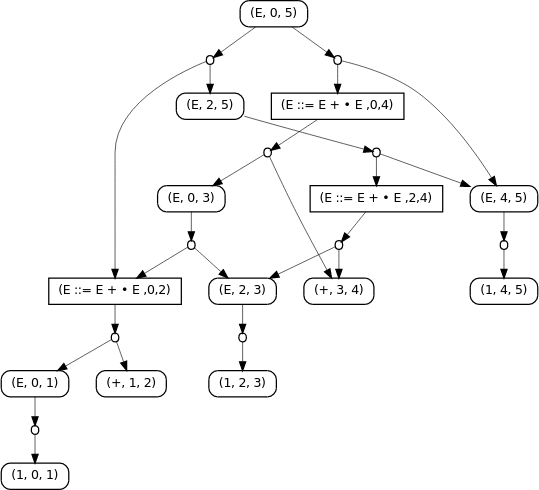
\includegraphics[scale=0.4]{images/sppf_example.png}}
    \end{column}
  \end{columns}
\end{frame}


\begin{frame}{Генерирование SPPF}
  \begin{itemize}
    \item Разбор графа с циклами потенциально может генерировать бесконечно много результатов
    \item Нужно представить результат такого разбора в виде конечной структуры --- SPPF
    \item Вместо результатов парсер будет генерировать узлы SPPF леса
    \item Узлы мемоизируются в процессе разбора
    \item Узлов конечное количество, поэтому разбор завершается
    \item Для извлечения результатов обходим SPPF
  \end{itemize}
\end{frame}


\begin{frame}{Пример SPPF для графа с циклом}
  \begin{columns}
    \begin{column}{0.2\textwidth}
      \raggedleft{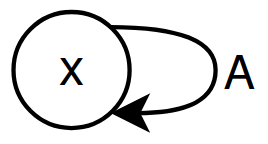
\includegraphics[scale=0.25]{images/graph_loop.png}}
    \end{column}
    \begin{column}{0.8\textwidth}
      \raggedright{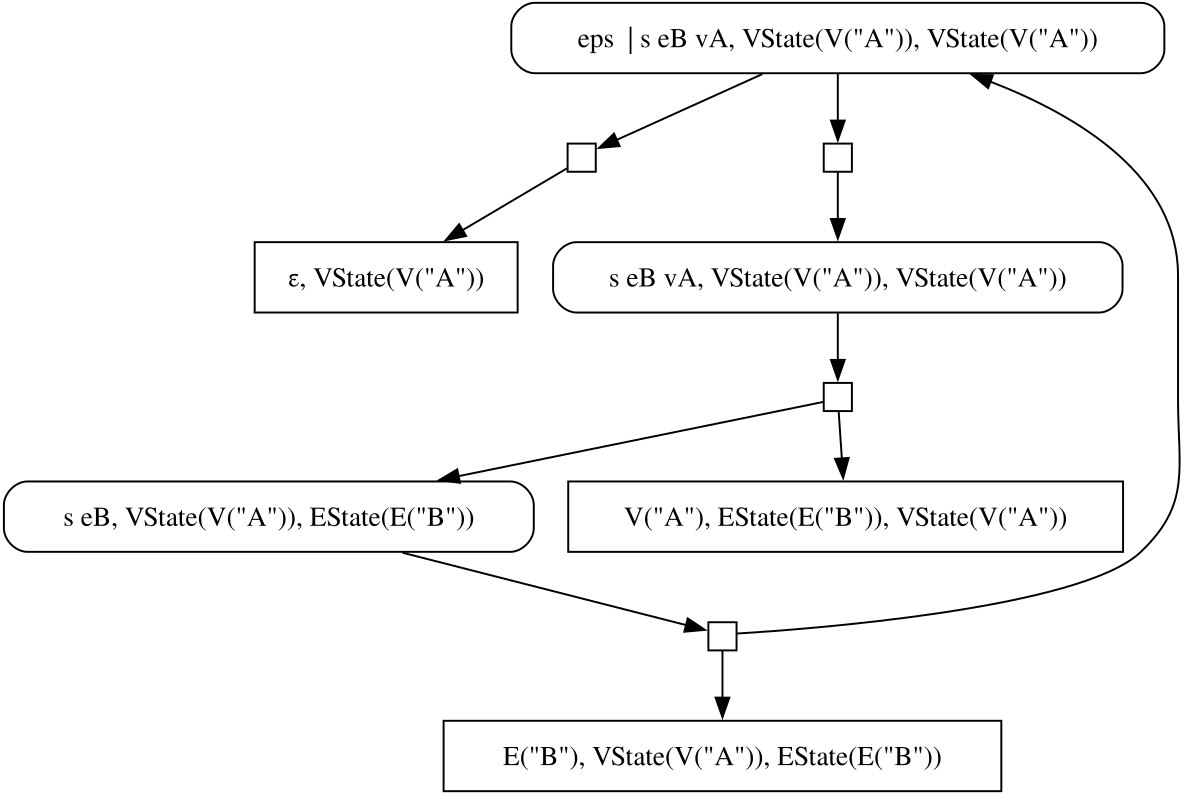
\includegraphics[scale=0.3]{images/sppf_loop.png}}
    \end{column}
  \end{columns}
\end{frame}


\begin{frame}{Исследование времени работы}
  Для исследования добавлена поддержка Neo4j.
  \vspace*{-0.5\baselineskip}
  \begin{table}[h]
    \renewcommand{\arraystretch}{1.1}
    \begin{tabular}{|b{0.21\linewidth}|b{0.16\linewidth}|b{0.16\linewidth}|b{0.15\linewidth}|b{0.15\linewidth}|}
      \hline
      \textbf{Граф}  & \textbf{Кол-во вершин} & \textbf{Кол-во рёбер} & \textbf{GParsers (мс)} & \textbf{Meerkat (мс)} \\
      \hline
      atom-primitive & 291        & 685        & \textbf{19.5} & 22.0 \\
      b.-m.-p.\footnote[1]{biomedical-mesure-primitive} & 341        & 711        & \textbf{23.5} & 42.5 \\
      generations    & 129        & 351        & \textbf{1.3}  & 1.4 \\
      pizza          & 671        & 2,604      & \textbf{61.4} & 123.9 \\
      \hline

      enzyme         & 48,815     & 86,543     & 121           & \textbf{116} \\
      eclass         & 239,111    & 360,248    & 1220          & \textbf{1095} \\
      go             & 582,929    & 1,437,437  & 6231          & \textbf{5367} \\
      go\_hierarchy  & 45,007     & 490,109    & 12015         & \textbf{8337} \\
      \hline
      yago           & 42,832,856 & 62,643,951 & \textbf{5558} & OOM \\
      \hline
    \end{tabular}
  \end{table}
\end{frame}


\begin{frame}{Результаты}
  \begin{itemize}
    \item Разработаны базовая структура парсера и комбинаторов, проверяющая корректность во время компиляции
    \item Поддержаны леворекурсивные и неоднозначные грамматики
    \item Поддержан разбор циклов в графе
    \item Реализована базовая поддержка Neo4j графов
    \item Проведено исследование времени работы: время сопоставимо с Meerkat
  \end{itemize}
\end{frame}


% --------- ДОП СЛАЙДЫ -------------
\appendix


\begin{frame}[fragile]{Сигнатуры комбинаторов}

  \begin{minted}[frame=single,fontsize=\footnotesize]{kotlin}
fun BaseParser<I, O1, R1>.seq(p2: BaseParser<O1, O2, R2>)
    : BaseParser<I, O2, Pair<R1, R2>>

fun BaseParser<I, O, R>.or(p2: BaseParser<I, O, R>)
    : BaseParser<I, O, R>

fun rule(first: BaseParser<I, O, R>, vararg rest: BaseParser<I, O, R>)

fun BaseParser<I, O, A>.using(f: (A) -> B): BaseParser<I, O, B>

fun BaseParser<I, O, R>.that(constraint: BaseParser<O, O2, R2>)
    : BaseParser<I, O, R> 
    
val BaseParser<S, S, R>.many: BaseParser<S, S, List<R>>
val BaseParser<S, S, R>.some: BaseParser<S, S, List<R>>
\end{minted}

\end{frame}

\begin{frame}[fragile]{Запросы для исследования времени (КС)}
  \begin{minted}[frame=single, fontsize=\footnotesize]{kotlin}
val subclassof1 = throughInE { it.label == "subClassOf" }
val subclassof = throughOutE { it.label == "subClassOf" }
val type1 = throughInE { it.label == "type" }
val type = throughOutE { it.label == "type" }
val Q1 = LazyParser<Neo4jVertexState, Neo4jVertexState, Any>()
Q1.p = (subclassof1 seq (Q1 or eps()) seq subclassof) or
        (type1 seq (Q1 or eps()) seq type)
\end{minted}
  \begin{minted}[frame=single, fontsize=\footnotesize]{scala}
val subclassof1: Symbol[L, N, _] = inE("subClassOf")
val subclassof: Symbol[L, N, _] = outE("subClassOf")
val type1: Symbol[L, N, _] = inE("type")
val _type: Symbol[L, N, _] = outE("type")
val grammar: Symbol[L, N, _] = 
  syn((subclassof1 ~ syn(grammar | ε) ~ subclassof) |
    (type1 ~ syn(grammar | ε) ~ _type))
\end{minted}


\end{frame}


\begin{frame}[fragile]{Запросы для исследования времени (yago)}
  \begin{minted}[frame=single,fontsize=\footnotesize]{text}
MATCH (x)-[:P74636308]->()-[:P59561600]->
()-[:P13305537*1..]->()-[:P92580544*1..]->
(:Entity{id:'40324616'}) RETURN DISTINCT x
\end{minted}

  \begin{minted}[frame=single,fontsize=\footnotesize]{kotlin}
(v { it.properties["id"] == "40324616" } seq
(inE { it.label == "P92580544" } seq inV()).some seq
(inE { it.label == "P13305537" } seq inV()).some seq
inE { it.label == "P59561600" } seq inV() seq
inE { it.label == "P74636308" } seq inV())
\end{minted}

  \begin{minted}[frame=single, fontsize=\footnotesize]{scala}
syn(V((e: Entity) => e.getProperty("id") == "40324616") ~
inE((e: Entity) => e.label() == "P92580544").+ ~
inE((e: Entity) => e.label() == "P13305537").+ ~
inE((e: Entity) => e.label() == "P59561600") ~
inE((e: Entity) => e.label() == "P74636308"))
  \end{minted}

\end{frame}






\end{document}

